\section{Desenvolvimento}

%%%%%%%%%%%%%%%%%%%%%%%%%%%%%%%%%%%%%%% Controle de Sistemas
\begin{frame}{Sistema de Controle}
\begin{block}{ Definição\tiny \cite{nise2009engenharia}}
"Um sistema de controle consiste em subsistemas e processos (ou plantas) constrídos com o objetivo de se obter uma saída desejada com desempenho desejado para uma entrada específica fornecida."
\end{block}
\begin{block}{ O paradigma }
A lógica clássica como paradigma na trascrição do mundo físico.
  %  O controle de sistema, bem como outras formas de transcrever o mundo físico, passam pelo paradigma da lógica clássica, cunhada por Aristóteles na forma lógica de lidar com o mundo.
\end{block}
\begin{block}{ A quebra do paradigma }
Questionamento e produção de ferramental para o tratamento de contradições e incertezas.
  %  No século XX o paradigma clássico foi questionado, procurando-se novas ferramentas para tratar questões que fogem das regras vigentes, como o tratamento de contradições e incertezas.
\end{block}

\end{frame}





%%%%%%%%%%%%%%%%%%%%%%%%%%%%%%%%%%%%%%% Lógica Clássica
\begin{frame}{Lógica Clássica \small - O paradigma}
\begin{block}{A origem \tiny \cite{JoaoInacio}}
Grécia Antiga : \emph{Tópicos} de Aristóteles  340 a.C.
\end{block}
\begin{block}{Princípios da Lógica \tiny \cite{JoaoInacio}}

\begin{enumerate}
\item Princípio de Identidade: 
    \begin{math}
	A \rightarrow A 
	\textrm{ ou } 
	\forall x(x=x);
    \end{math}

\item Princípio do Terceiro Excluído:
    \begin{math}
	A \vee \neg A
	\textrm{ ou }
	\forall x(Ax \vee \neg Ax);
    \end{math}

\item Princípio da Não Contradição: 
    \begin{math}
	\neg (A \wedge \neg A)
	\textrm{ ou }
	\forall x\neg(Ax \wedge \neg Ax).
    \end{math}

\end{enumerate}

\end{block}
\end{frame}





%%%%%%%%%%%%%%%%%%%%%%%%%%%%%%%%%%%%%%% Lógica Paraconsistente
\begin{frame}{Lógica Paraconsistente - \small A quebra do paradigma}

\begin{block}{Criadores \tiny \cite{DecioKrause}}
\begin{itemize}
\item Newton Carneiro Affonso da Costa (1929-presente data)
\item Stanislaw Jaskiwski (1906-1965)
\end{itemize}
\end{block}

\begin{block}{Desenvolvimento: Costa, Subrahmanian e Vago \tiny \cite{DecioKrause}}
\begin{itemize}
\item Lógica Paraconsistente Anotada
\item extensão a uma Lógica de Predicados Paraconsistente Anotada de primeira ordem 
\end{itemize}
\end{block}

\end{frame}





%%%%%%%%%%%%%%%%%%%%%%%%%%%%%%%%%%%%%%% Proposição
\begin{frame}{A Proposição}
\vspace{1cm}

\begin{block}{}
\center
Para toda \textbf{proposição $P$} há um par de valores, \\
chamada de \textbf{anotação}, \textbf{$(\mu , \lambda )$}, onde \\
$\mu$ é o \textbf{grau de evidência favorável} e \\
$\lambda $ é o \textbf{grau de evidência desfavorável}, \\
representada como  \textbf{$P_{( \mu , \lambda )}$ }.
\end{block}

\end{frame}





%%%%%%%%%%%%%%%%%%%%%%%%%%%%%%%%%%%%%%% Lógica Paraconsistente Anotada
\begin{frame}{Lógica Paraconsistente Anotada Evidencial $\tau$ (LPA$E\tau$) \tiny \cite{JoaoInacio}}

\begin{block}{
\centering 
$\tau = \{ ( \mu , \lambda ) \mid \mu ,\lambda \in [0,1] \subset \Re \}$
}
\end{block}
\vspace{0.4cm}
\begin{minipage}{0.40\linewidth}
\begin{figure}[!htb]
%\caption{Reticulado finito de Hasse}
\center\includegraphics[scale=0.6]{./imagens/C421reticuladoHasse.eps}
\label{fig:reticuladoHasse}
%%%{\small Fonte: \cite{JoaoInacio} }
\end{figure}
\end{minipage}
\begin{minipage}{0.55\linewidth}
\center
\begin{itemize}
\item $(0,0) = \bot \Rightarrow $ Paracompleto;
\item $(0,1) = F \Rightarrow $ Falso;
\item $(1,1) = \top \Rightarrow $ Contradição;
\item $(1,0) = V \Rightarrow $ Verdade.
\end{itemize}
\end{minipage}

\end{frame}





%%%%%%%%%%%%%%%%%%%%%%%%%%%%%%%%%%%%%%% Quadrado Unitário no Plano Cartesiano
\begin{frame}{Quadrado Unitário no Plano Cartesiano}

\begin{block}{ \centering   $(\mu, \lambda ) \leftrightarrow (x,y) $ } \end{block}
\vspace{1cm}
\begin{minipage}{0.40\linewidth}
\begin{figure}[!htb]
%\caption{Representação do reticulado no quadrado unitário no plano cartesiano}
\center\includegraphics[scale=1.0]{./imagens/C422qupc.eps}
\label{fig:reticuladoQUPC}
%%%{\small Fonte: \cite{JoaoInacio} }
\end{figure}
\end{minipage}
\begin{minipage}{0.55\linewidth}
\center
\begin{itemize}
\item $A: (0,0) = \bot \Rightarrow $ Paracompleto;
\item $B: (0,1) = F \Rightarrow $ Falso;
\item $C: (1,1) = \top \Rightarrow $ Contradição;
\item $D: (1,0) = V \Rightarrow $ Verdade.
\end{itemize}
\end{minipage}

\end{frame}

%%%%%%%%%%%%%%%%%%%%%%%%%%%%%%%%%%%%%%% Reta Perfeitamente Definida
\begin{frame}{Reta Perfeitamente Definida}
\begin{block}{ \centering   $(\mu, \lambda ) \leftrightarrow (x,y) $ } \end{block}
\vspace{1cm}
\begin{minipage}{0.50\linewidth}
\begin{figure}[!htb]
%\caption{Representação da Reta Perfeitamente Definida}
\center\includegraphics[scale=1.0]{./imagens/C424retaPerfeitamenteDefinida.eps}
%\label{fig:retaPerfeitamenteDefinida}
%%%{\small Fonte: \cite{JoaoInacio} }
\end{figure}
\end{minipage}
\begin{minipage}{0.45\linewidth}

\begin{itemize}
\item $\mu + \lambda = 1$
\item $\mu + \lambda - 1 = 0$
\item Grau de contradição
  \begin{itemize}
    \item $G _{ct} = \mu + \lambda - 1$
    \item $-1 \leqslant G _{ct} \leqslant 1$
  \end{itemize}
\end{itemize}
\end{minipage}

\end{frame}

%%%%%%%%%%%%%%%%%%%%%%%%%%%%%%%%%%%%%%% Reta Perfeitamente Indefinida
\begin{frame}{Reta Perfeitamente Indefinida}
\begin{block}{ \centering   $(\mu, \lambda ) \leftrightarrow (x,y) $ } \end{block}
\vspace{1cm}
\begin{minipage}{0.50\linewidth}
\begin{figure}[!htb]
%\caption{Representação da Reta Perfeitamente Indefinida}
\center\includegraphics[scale=1.0]{./imagens/C426retaPerfeitamenteIndefinida.eps}
%\label{fig:retaPerfeitamenteDefinida}
%%%{\small Fonte: \cite{JoaoInacio} }
\end{figure}
\end{minipage}
\begin{minipage}{0.45\linewidth}

\begin{itemize}
\item $\mu - \lambda = 0$
\item Grau de certeza
  \begin{itemize}
    \item $G _{c} = \mu - \lambda$
    \item $-1 \leqslant G _{c} \leqslant 1$
  \end{itemize}
\end{itemize}
\end{minipage}

\end{frame}

%%%%%%%%%%%%%%%%%%%%%%%%%%%%%%%%%%%%%%% Representação do reticulado
\begin{frame}{Representação do Reticulado da LPA$E\tau$ {\small subdividido em 12 regiões}}
\vspace{1cm}
\begin{minipage}{0.50\linewidth}
\begin{figure}[!htb]
%\caption{Representação dos valores de controle}
\center\includegraphics[scale=0.65]{./imagens/C428retasgcgct.eps}
\end{figure}
\end{minipage}
\begin{minipage}{0.45\linewidth}
\begin{figure}[!htb]
\center\includegraphics[scale=0.65]{./imagens/C430gcgct.eps}
%\caption{Representação do reticulado da LPA2v subdividido em 12 regiões}
\label{fig:reticuladoLPA2v}
\end{figure}
\end{minipage}

\end{frame}












%%%%%%%%%%%%%%%%%%%%%%%%%%%%%%%%%%%%%%% A proposição e a anotação
\begin{frame}{A proposição e a anotação}

\begin{exampleblock}{ A proposição }
  P : A velocidade de rotação é máxima.    
\end{exampleblock}
\begin{block}{ A anotação }
  \begin{itemize}
    \item Grau de evidência favorável 0 ($\mu_0$): Valor de referência;
    \item Grau de evidência favorável 1 ($\mu_1$): Valor da variável controlada.
      \begin{itemize}
        \item $\mu_1 = 1 - \lambda$
      \end{itemize}
  \end{itemize}
\end{block}
\end{frame}





%%%%%%%%%%%%%%%%%%%%%%%%%%%%%%%%%%%%%%% Diagrama de blocos do controle utilizando a LPAEt
\begin{frame}{Diagrama de blocos do controle utilizando a LPA$E\tau$}

\begin{figure}[!h]%%%%%%%%%%%%%%%%%%%%%%%%%%%%%%%%fg
\centering
%\caption{Diagrama de blocos do controle utilizando a LPA$E\tau$}
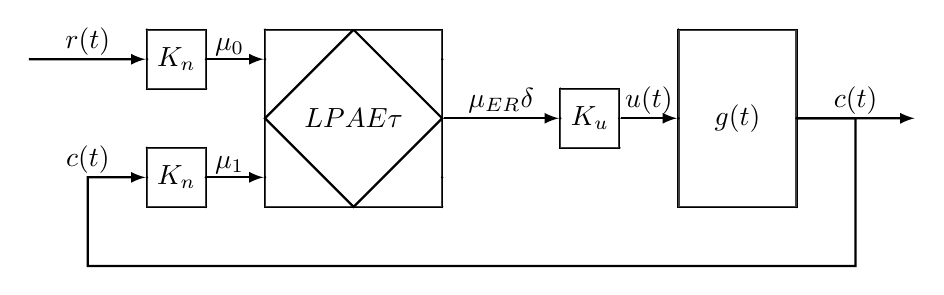
\begin{tikzpicture}[scale=0.75]
\tikzset{ >=latex, inner sep=0pt, outer sep=0pt,  }

%\draw [lightgray, dashed](0,0) grid (15,4.2);

%%% Blocos 

% Kn normalização rps -> 0..1
\node [fill=black, circle] (KSP0) at (2.0,4.0) { };
\node [fill=black, circle] (KSP1) at (3.0,3.0) { };
\draw[thick] (KSP0) rectangle (KSP1);
\fill[white, nearly transparent] (KSP0) rectangle (KSP1);
\node [fill=black, circle] (KSPin)  at (2.0,3.5) { }; 
\node [fill=black, circle] (KSPout) at (3.0,3.5) { }; 
\node (Kn1) at (2.5,3.5) {$K_n$};

% Kn Sensor
\node [fill=black, circle] (KS0) at (2.0,2.0) { };
\node [fill=black, circle] (KS1) at (3.0,1.0) { };
\draw[thick] (KS0) rectangle (KS1);
\fill[white, nearly transparent] (KS0) rectangle (KS1);
\node [fill=black, circle] (KSin)  at (2.0,1.5) { };
\node [fill=black, circle] (KSout) at (3.0,1.5) { };
\node (Kn2) at (2.5,1.5) {$K_n$};

% LPAEt
\node [fill=black, circle] (LPA0) at (4,4.0) { };
\node [fill=black, circle] (LPA1) at (7,1.0) { };
\draw[thick] (LPA0) rectangle (LPA1);
\fill[white, nearly transparent] (LPA0) rectangle (LPA1);
\draw [thick] (5.5,4.0) -- (7.0,2.5) -- (5.5,1.0) -- (4.0,2.5) -- (5.5,4.0);
\node (LPA2v) at (5.5,2.5) {$LPAE\tau$};
\node [fill=black, circle] (LPAu0)  at (4.0,3.5) { };
\node [fill=black, circle] (LPAu1)  at (4.0,1.5) { };
\node [fill=black, circle] (LPAgc)  at (7.0,3.5) { };
\node [fill=black, circle] (LPAs)   at (7.0,2.5) { };
\node [fill=black, circle] (LPAgct) at (7.0,1.5) { };
\node (LPA2vu0)  at (3.4,3.7) {$\mu _0$};
\node (LPA2vu1)  at (3.4,1.7) {$\mu _1$};

% Ku u(t)
\node [fill=black, circle] (KU0) at ( 9.0,3.0) { };
\node [fill=black, circle] (KU1) at (10.0,2.0) { };
\draw[thick] (KU0) rectangle (KU1);
\fill[white, nearly transparent] (KU0) rectangle (KU1);
\node [fill=black, circle] (KUin)  at (9.0,2.5) { };
\node [fill=black, circle] (KUout) at (10.0,2.5) { };
\node (Ku2) at (9.5,2.5) {$K_u$};


% Planta
\node [fill=black, circle] (GT0) at (11,4.0) { };
\node [fill=black, circle] (GT1) at (13,1.0) { };
\draw[thick] (GT0) rectangle (GT1);
\fill[white, nearly transparent] (GT0) rectangle (GT1);
\node [fill=black, circle] (GTin)  at (11.0,2.5) { };
\node [fill=black, circle] (GTout) at (13.0,2.5) { };
\node (planta) at (12.0,2.5) {$g(t)$};



%%% Linhas 

% set point
\draw [->, thick] (0.0,3.5) -- (KSPin);
\node (rt) at (1.0,3.8) {$r(t)$};

% GT -> fim
\draw [->, thick] (GTout) -- (15,2.5);
\node (ct) at (14.0,2.8) {$c(t)$};
\node (ct) at (1.0,1.8) {$c(t)$};

% normalização 0..1 -> LPA2v u0
\draw [->, thick] (KSPout) -- (LPAu0);

% normalização 0..1 -> LPA2v u1
\draw [->, thick] (KSout) -- (LPAu1);

% LPAEt -> Ku
\draw [->, thick] (LPAs) -- (KUin);
\node (ut) at (8.0,2.8) {$\mu_{ER}\delta$};

% Ku -> GT
\draw [->, thick] (KUout) -- (GTin);
\node (ut) at (10.5,2.8) {$u(t)$};

% GT -> Kn Sensor
\draw [->, thick] (GTout) -- (14.0,2.5) -- (14.0,0.0) -- (1.0,0.0) -- (1.0,1.5) -- (KSin);


\end{tikzpicture}
\label{fig:diagramaBlocosLPAEt}

{\vspace{0.2cm} \small Fonte: Próprio autor}
\end{figure}
%%%%%%%%%%%%%%%%%%%%%%%%%%%%%%%%%%%%%%%%


\end{frame}








%%%%%%%%%%%%%%%%%%%%%%%%%%%%%%%%%%%%%%% Representação do reticulado da LPAEt para ação de controle Liga-Desliga
\begin{frame}{ Representação do reticulado da LPA$E\tau$ {\small dividido em duas partes} }

%%%%%%%%%%%%%%%%%%%%%%%%%%%%%%%%%%%%%%%%%%%%%%% Fg
\begin{figure}[!htb]%%%%%%%%%%%%%%%%%%%%%%%%%%%%%%
\centering
%\caption{Representação do reticulado da LPA$E\tau$ para ação de controle Liga-Desliga}
\subfloat[$Gct$ positivo ($\mu_0 > \mu_1$)]{\label{fig:gctpos}

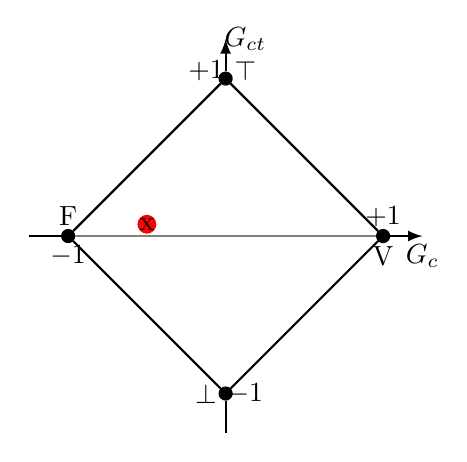
\begin{tikzpicture}[scale=0.5]
\tikzset{ >=latex, inner sep=0pt, outer sep=0pt,  }
%\draw [lightgray, dashed](0,0) grid (10,10);

\node [fill=black, circle] (V) at (9,5) {:};
\node [fill=black, circle] (F) at (1,5) {:};
\node [fill=black, circle] (T) at (5,9) {:};
\node [fill=black, circle] (L) at (5,1) {:};

\draw [->, thick] (V)   -- (10,5);
\draw [    thick] (0,5) -- (F);
\draw [->, thick] (T)   -- (5,10);
\draw [    thick] (5,0) -- (L);

\draw [thick] (V) -- (T);
\draw [thick] (T) -- (F);
\draw [thick] (F) -- (L);
\draw [thick] (L) -- (V);

\draw [gray,thick] (V) -- (F);

\node at (10,4.5) {$G_{c}$};
\node at (5.5,10) {$G_{ct}$};

\node at (4.5,9.2) {$+1$};
\node at (9.0,5.5) {$+1$};
\node at (5.5,1.0) {$-1$};
\node at (1.0,4.5) {$-1$};

\node at (9.0,4.5) {V};
\node at (1.0,5.5) {F};
\node at (5.5,9.2) {$\top$};
\node at (4.5,1.0) {$\bot$};

\node [fill=red, circle] (MU) at (3.0,5.3) {x};

\end{tikzpicture} }
\subfloat[$Gct$ negativo ($\mu_0<\mu_1$)]{\label{fig:gctneg}
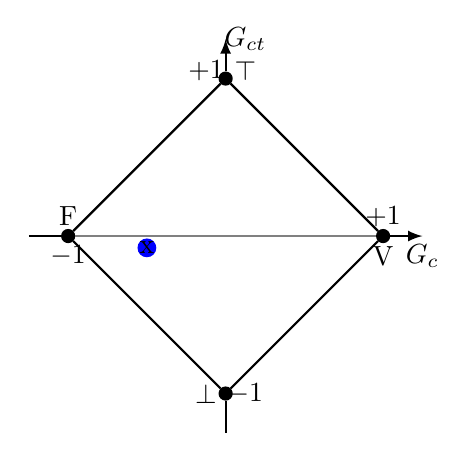
\begin{tikzpicture}[scale=0.5]
\tikzset{ >=latex, inner sep=0pt, outer sep=0pt,  }
%\draw [lightgray, dashed](0,0) grid (10,10);

\node [fill=black, circle] (V) at (9,5) {:};
\node [fill=black, circle] (F) at (1,5) {:};
\node [fill=black, circle] (T) at (5,9) {:};
\node [fill=black, circle] (L) at (5,1) {:};

\draw [->, thick] (V)   -- (10,5);
\draw [    thick] (0,5) -- (F);
\draw [->, thick] (T)   -- (5,10);
\draw [    thick] (5,0) -- (L);

\draw [thick] (V) -- (T);
\draw [thick] (T) -- (F);
\draw [thick] (F) -- (L);
\draw [thick] (L) -- (V);

\draw [gray,thick] (V) -- (F);

\node at (10,4.5) {$G_{c}$};
\node at (5.5,10) {$G_{ct}$};

\node at (4.5,9.2) {$+1$};
\node at (9.0,5.5) {$+1$};
\node at (5.5,1.0) {$-1$};
\node at (1.0,4.5) {$-1$};

\node at (9.0,4.5) {V};
\node at (1.0,5.5) {F};
\node at (5.5,9.2) {$\top$};
\node at (4.5,1.0) {$\bot$};

\node [fill=blue, circle] (MU1) at (3.0,4.7) {x};

\end{tikzpicture}}

\label{fig:sistPrimeiraOrdem}

{\small Fonte: Próprio autor}
\end{figure}%%%%%%%%%%%%%%%%%%%%%%%%%%%%%%%%%%%%%%
%%%%%%%%%%%%%%%%%%%%%%%%%%%%%%%%%%%%%%%%%%%%%%%%%%
\end{frame}






%%%%%%%%%%%%%%%%%%%%%%%%%%%%%%%%%%%%%%% Representação do reticulado da LPAEt dividido em duas partes
\begin{frame}{Região de controle Liga-Desliga no reticulado da LPA$E\tau$ }

%%%%%%%%%%%%%%%%%%%%%%%%%%%%%%%%%%%%%%%%%%%%%%%%%%%%
\begin{figure}[!h]%%%%%%%%%%%%%%%%%%%%%%%%%%%%%%%%fg
\centering
%\caption{Representação do reticulado da LPA$E\tau$ dividido em duas partes}
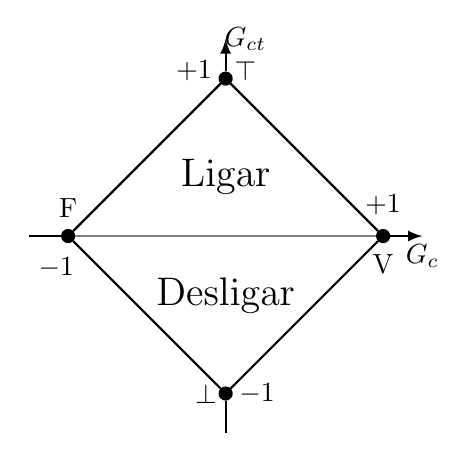
\begin{tikzpicture}[scale=0.50]
\tikzset{ >=latex, inner sep=0pt, outer sep=0pt,  }

%\draw [lightgray, dashed](0,0) grid (10,10);

\node [fill=black, circle] (V) at (9,5) {:};
\node [fill=black, circle] (F) at (1,5) {:};
\node [fill=black, circle] (T) at (5,9) {:};
\node [fill=black, circle] (L) at (5,1) {:};

\draw [->, thick] (V)   -- (10,5);
\draw [    thick] (0,5) -- (F);
\draw [->, thick] (T)   -- (5,10);
\draw [    thick] (5,0) -- (L);

\draw [thick] (V) -- (T);
\draw [thick] (T) -- (F);
\draw [thick] (F) -- (L);
\draw [thick] (L) -- (V);

\draw [gray,thick] (V) -- (F);

\node at (10,4.5) {$G_{c}$};
\node at (5.5,10) {$G_{ct}$};

\node at (4.2,9.2) {$+1$};
\node at (9.0,5.8) {$+1$};
\node at (5.8,1.0) {$-1$};
\node at (0.7,4.2) {$-1$};

\node at (9.0,4.3) {V};
\node at (1.0,5.7) {F};
\node at (5.5,9.2) {$\top$};
\node at (4.5,1.0) {$\bot$};

\node at (5.0,6.5) {\Large{Ligar}};
\node at (5.0,3.5) {\Large{Desligar}};

\end{tikzpicture}
\label{fig:reticuladoEtOnOff}

{\small Fonte: Próprio autor }
\end{figure}%%%%%%%%%%%%%%%%%%%%%%%%%%%%%%%%%%%%%%
%%%%%%%%%%%%%%%%%%%%%%%%%%%%%%%%%%%%%%%%%%%%%%%%%%

  
\end{frame}









%%%%%%%%%%%%%%%%%%%%%%%%%%%%%%%%%% Representação da zona morta no reticulado da LPAEt
\begin{frame}{ Região de zona morta no reticulado da LPA$E\tau$}
%%%%%%%%%%%%%%%%%%%%%%%%%%%%%%%%%%%%%%%%%%%%%%%%%%%%%%%%% Fg
\begin{figure}[!h]%%%%%%%%%%%%%%%%%%%%%%%%%%%%%%%%%%%%%%%%%%
\centering
%\caption{Representação da zona morta no reticulado da LPA$E\tau$}
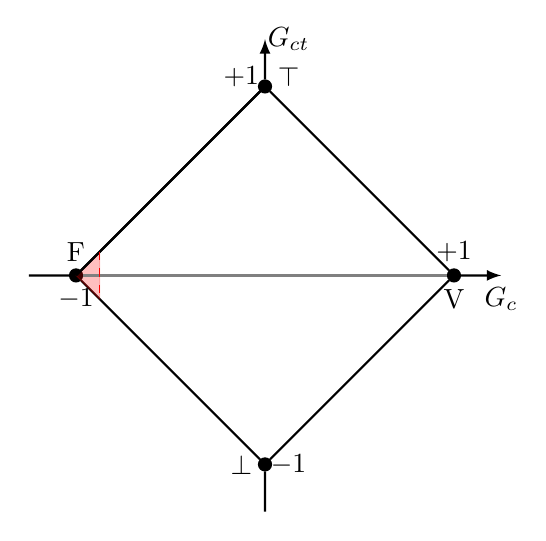
\begin{tikzpicture}[scale=0.60]
\tikzset{ >=latex, inner sep=0pt, outer sep=0pt,  }

%\draw [lightgray, dashed](0,0) grid (10,10);

\node [fill=black, circle] (V) at (9,5) {:};
\node [fill=black, circle] (F) at (1,5) {:};
\node [fill=black, circle] (T) at (5,9) {:};
\node [fill=black, circle] (L) at (5,1) {:};

\draw [->, thick] (V)   -- (10,5);
\draw [    thick] (0,5) -- (F);
\draw [->, thick] (T)   -- (5,10);
\draw [    thick] (5,0) -- (L);

\draw [thick] (V) -- (T);
\draw [thick] (T) -- (F);
\draw [thick] (F) -- (L);
\draw [thick] (L) -- (V);

\node at (10,4.5) {$G_{c}$};
\node at (5.5,10) {$G_{ct}$};

\node at (4.5,9.2) {$+1$};
\node at (9.0,5.5) {$+1$};
\node at (5.5,1.0) {$-1$};
\node at (1.0,4.5) {$-1$};

\node at (9.0,4.5) {V};
\node at (1.0,5.5) {F};
\node at (5.5,9.2) {$\top$};
\node at (4.5,1.0) {$\bot$};

\draw [fill, red,nearly transparent] (1.0,5.0) -- (1.5,5.5) -- (1.5,4.5) -- (1.0,5.0);
\draw [thick] (5.0,9.0) -- (1.0,5.0);
\draw [gray,thick] (V) -- (F);
\draw [dashed, red] (1.5,5.5) -- (1.5,4.5);
\end{tikzpicture}
\label{fig:zonaMorta}

{\small Fonte: Próprio autor }
\end{figure}
%%%%%%%%%%%%%%%%%%%%%%%%%%%%%%%%%%%%%%%%%%%%%%%%%%%%%%%%%%%%
 
\end{frame}






%%%%%%%%%%%%%%%%%%%%%%%%%%%%%%%%%%%%%%% Representação da região de travamento no reticulado da LPAEt
\begin{frame}{Região de travamento no reticulado da LPA$E\tau$}
%%%%%%%%%%%%%%%%%%%%%%%%%%%%%%%%%%%%%%%%%%%%%%% Fg
\begin{figure}[!h]%%%%%%%%%%%%%%%%%%%%%%%%%%%%%%%%
\centering
%\caption{Representação da região de travamento no reticulado da LPA$E\tau$}
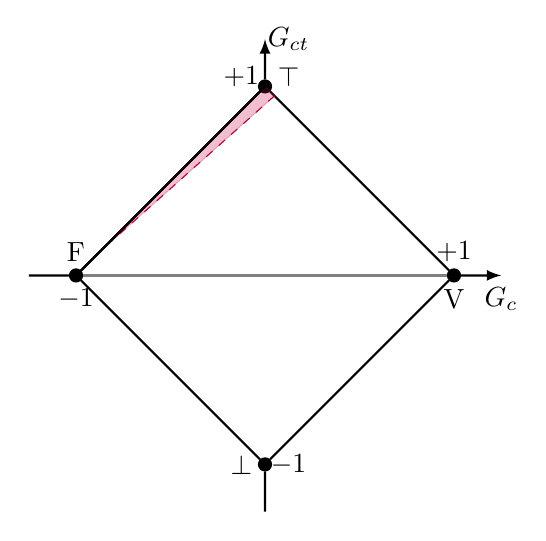
\begin{tikzpicture}[scale=0.60]
\tikzset{ >=latex, inner sep=0pt, outer sep=0pt,  }

%\draw [lightgray, dashed](0,0) grid (10,10);

\node [fill=black, circle] (V) at (9,5) {:};
\node [fill=black, circle] (F) at (1,5) {:};
\node [fill=black, circle] (T) at (5,9) {:};
\node [fill=black, circle] (L) at (5,1) {:};

\draw [->, thick] (V)   -- (10,5);
\draw [    thick] (0,5) -- (F);
\draw [->, thick] (T)   -- (5,10);
\draw [    thick] (5,0) -- (L);

\draw [thick] (V) -- (T);
\draw [thick] (T) -- (F);
\draw [thick] (F) -- (L);
\draw [thick] (L) -- (V);

\node at (10,4.5) {$G_{c}$};
\node at (5.5,10) {$G_{ct}$};

\node at (4.5,9.2) {$+1$};
\node at (9.0,5.5) {$+1$};
\node at (5.5,1.0) {$-1$};
\node at (1.0,4.5) {$-1$};

\node at (9.0,4.5) {V};
\node at (1.0,5.5) {F};
\node at (5.5,9.2) {$\top$};
\node at (4.5,1.0) {$\bot$};

\draw [fill, purple, nearly transparent] (1.5,5.5) -- (5.0,9.0) -- (5.2,8.8) -- (1.5,5.5);
\draw [dashed, purple] (5.2,8.8) -- (1.5,5.5);
\draw [thick] (5.0,9.0) -- (1.0,5.0);
\draw [gray,thick] (V) -- (F);
\end{tikzpicture}
\label{fig:travamentoEixo}

{\small Fonte: Próprio autor }
\end{figure}
%%%%%%%%%%%%%%%%%%%%%%%%%%%%%%%%%%%%%%%%%%%%%%%%%%
\end{frame}








%%%%%%%%%%%%%%%%%%%%%%%%%%%%%%%%%%%%%%% Representação da região ativa no reticulado da LPAEt
\begin{frame}{Região ativa no reticulado da LPA$E\tau$}
%%%%%%%%%%%%%%%%%%%%%%%%%%%%%%%%%%%%%%%%%%%%%%% Fg
\begin{figure}[!h]%%%%%%%%%%%%%%%%%%%%%%%%%%%%%%%%
\centering
%\caption{Representação da região ativa no reticulado da LPA$E\tau$}
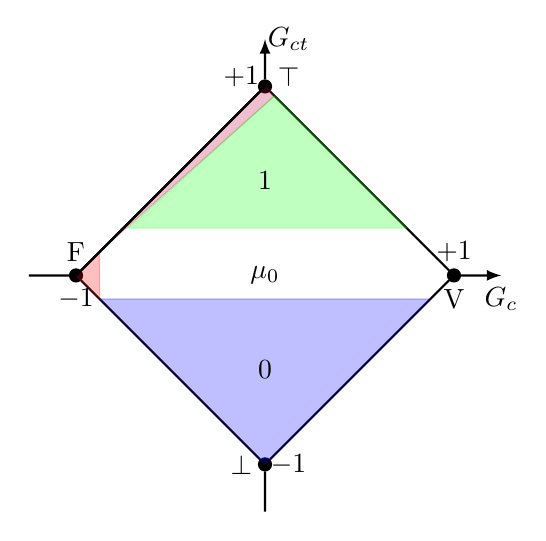
\begin{tikzpicture}[scale=0.60]
\tikzset{ >=latex, inner sep=0pt, outer sep=0pt,  }

%\draw [lightgray, dashed](0,0) grid (10,10);

\node [fill=black, circle] (V) at (9,5) {:};
\node [fill=black, circle] (F) at (1,5) {:};
\node [fill=black, circle] (T) at (5,9) {:};
\node [fill=black, circle] (L) at (5,1) {:};

\draw [->, thick] (V)   -- (10,5);
\draw [    thick] (0,5) -- (F);
\draw [->, thick] (T)   -- (5,10);
\draw [    thick] (5,0) -- (L);

\draw [thick] (V) -- (T);
\draw [thick] (T) -- (F);
\draw [thick] (F) -- (L);
\draw [thick] (L) -- (V);

\node at (10,4.5) {$G_{c}$};
\node at (5.5,10) {$G_{ct}$};

\node at (4.5,9.2) {$+1$};
\node at (9.0,5.5) {$+1$};
\node at (5.5,1.0) {$-1$};
\node at (1.0,4.5) {$-1$};

\node at (9.0,4.5) {V};
\node at (1.0,5.5) {F};
\node at (5.5,9.2) {$\top$};
\node at (4.5,1.0) {$\bot$};

\draw [fill, red,nearly transparent] (1.0,5.0) -- (1.5,5.5) -- (1.5,4.5) -- (1.0,5.0);
\draw [fill, purple, nearly transparent] (1.5,5.5) -- (5.0,9.0) -- (5.2,8.8) -- (1.5,5.5);
\draw [fill, blue, nearly transparent] (5.0,1.0) -- (8.5,4.5) -- (1.5,4.5) -- (5.0,1.0);
\draw [fill, green, nearly transparent] (5.2,8.8) -- (2.1,6.0) -- (8.0,6.0) -- (5.2,8.8);

\draw [thick] (5.0,9.0) -- (1.0,5.0);

\node at (5.0,7.0) {1};
\node at (5.0,5.0) {$\mu_0$};
\node at (5.0,3.0) {0};

\end{tikzpicture}
\label{fig:regiaoAtiva}

{\small Fonte: Próprio autor }
\end{figure}
%%%%%%%%%%%%%%%%%%%%%%%%%%%%%%%%%%%%%%%%%%%%%%%%%%

\end{frame}







%%%%%%%%%%%%%%%%%%%%%%%%%%%%%%%%%%%%%%% Representação da região ativa no reticulado da LPAEt
\begin{frame}{Região ativa no reticulado da LPA$E\tau$}
%%%%%%%%%%%%%%%%%%%%%%%%%%%%%%%%%%%%%%%%%%%%%% Fig
\begin{figure}[!h]%%%%%%%%%%%%%%%%%%%%%%%%%%%%%%%%
\centering
%\caption{Representação da região ativa no reticulado da LPA$E\tau$}
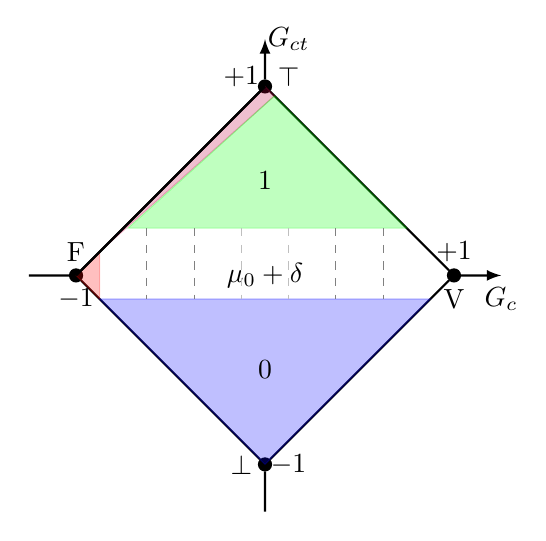
\begin{tikzpicture}[scale=0.60]
\tikzset{ >=latex, inner sep=0pt, outer sep=0pt,  }

%\draw [lightgray, dashed](0,0) grid (10,10);

\node [fill=black, circle] (V) at (9,5) {:};
\node [fill=black, circle] (F) at (1,5) {:};
\node [fill=black, circle] (T) at (5,9) {:};
\node [fill=black, circle] (L) at (5,1) {:};

\draw [->, thick] (V)   -- (10,5);
\draw [    thick] (0,5) -- (F);
\draw [->, thick] (T)   -- (5,10);
\draw [    thick] (5,0) -- (L);

\draw [thick] (V) -- (T);
\draw [thick] (T) -- (F);
\draw [thick] (F) -- (L);
\draw [thick] (L) -- (V);

\node at (10,4.5) {$G_{c}$};
\node at (5.5,10) {$G_{ct}$};

\node at (4.5,9.2) {$+1$};
\node at (9.0,5.5) {$+1$};
\node at (5.5,1.0) {$-1$};
\node at (1.0,4.5) {$-1$};

\node at (9.0,4.5) {V};
\node at (1.0,5.5) {F};
\node at (5.5,9.2) {$\top$};
\node at (4.5,1.0) {$\bot$};

\draw [fill, red,nearly transparent] (1.0,5.0) -- (1.5,5.5) -- (1.5,4.5) -- (1.0,5.0);
\draw [fill, purple, nearly transparent] (1.5,5.5) -- (5.0,9.0) -- (5.2,8.8) -- (1.5,5.5);
\draw [fill, blue, nearly transparent] (5.0,1.0) -- (8.5,4.5) -- (1.5,4.5) -- (5.0,1.0);
\draw [fill, green, nearly transparent] (5.2,8.8) -- (2.1,6.0) -- (8.0,6.0) -- (5.2,8.8);

\draw [thick] (5.0,9.0) -- (1.0,5.0);

\node at (5.0,7.0) {1};
\node at (5.0,5.0) {$\mu_0 + \delta$};
\node at (5.0,3.0) {0};

\draw [dashed, gray] (2.5,6.0) -- (2.5,4.5);
\draw [dashed, gray] (3.5,6.0) -- (3.5,4.5);
\draw [dashed, gray] (6.5,6.0) -- (6.5,4.5);
\draw [dashed, gray] (7.5,6.0) -- (7.5,4.5);
\draw [dashed, lightgray] (4.5,6.0) -- (4.5,4.5);
\draw [dashed, lightgray] (5.5,6.0) -- (5.5,4.5);

\end{tikzpicture}
\label{fig:regiaoAtivaMuDelta}

{\small Fonte: Próprio autor }
\end{figure}
%%%%%%%%%%%%%%%%%%%%%%%%%%%%%%%%%%%%%%%%%%%%%%%%%%

\end{frame}






%%%%%%%%%%%%%%%%%%%%%%%%%%%%%%%%%%%%%%% Valores de correção para a condição de contradição
\begin{frame}{Valores de correção para a condição de contradição}

\begin{table}[h]
\centering
%\caption{Valores de correção para a condição de contradição}
\label{tab:correcaoDelta}

\begin{tabular}{c|c|c||c}
\hline
%Intervalo de amostras  &  erro médio relativo \\ \hline
Limite Inferior & Alvo & Limite Superior & Valor de Correção\\ \hline
\hline
%0 a 1 $\tau$ & 83,40 \% \\ \hline
 9,5 & 10 & 10,5 & $\delta_0$ \\ \hline
10,5 & 11 & 11,5 & $\delta_1$ \\ \hline
11,5 & 12 & 12,5 & $\delta_2$ \\ \hline
12,5 & 13 & 14,0 & $\delta_3$ \\ \hline
14,0 & 15 & 15,5 & $\delta_4$ \\ \hline
15,5 & 16 & 17,0 & $\delta_5$ \\ \hline
17,0 & 18 & 19,0 & $\delta_6$ \\ \hline
19,0 & 20 & 21,0 & $\delta_7$ \\ \hline
21,0 & 22 & 23,0 & $\delta_8$ \\ \hline
23,4 & 24 & 25,4 & $\delta_9$ \\ \hline
25,4 & 27 & 28,4 & $\delta_{10}$ \\ \hline
28,4 & 30 & 31,4 & $\delta_{11}$ \\ \hline

\end{tabular}
{\vspace{-0.2cm} \small Fonte: Próprio autor}
\end{table}

\end{frame}
%%%%%%%%%%%%%%%%%%%%%%%%%%%%%%%%%%%%%%% Valores de correção para a condição de contradição
\begin{frame}{Valores de correção para a condição de contradição}

\begin{table}[h]
\centering
%\caption{Valores de correção para a condição de contradição}
\label{tab:correcaoDelta}

\begin{tabular}{c|c|c||c}
\hline
%Intervalo de amostras  &  erro médio relativo \\ \hline
Limite Inferior & Alvo & Limite Superior & Valor de Correção\\ \hline
\hline
%0 a 1 $\tau$ & 83,40 \% \\ \hline
31,4 & 33 & 34,4 & $\delta_{12}$ \\ \hline
34,4 & 36 & 37,4 & $\delta_{13}$ \\ \hline
37,4 & 39 & 40,9 & $\delta_{14}$ \\ \hline
40,9 & 43 & 44,9 & $\delta_{15}$ \\ \hline
44,9 & 47 & 48,9 & $\delta_{16}$ \\ \hline
48,9 & 51 & 53,4 & $\delta_{17}$ \\ \hline
53,4 & 56 & 58,9 & $\delta_{18}$ \\ \hline
58,9 & 62 & 64,9 & $\delta_{19}$ \\ \hline
64,9 & 68 & 71,3 & $\delta_{20}$ \\ \hline
71,3 & 75 & 78,3 & $\delta_{21}$ \\ \hline
78,3 & 82 & 86,3 & $\delta_{22}$ \\ \hline
86,3 & 91 &100,0 & $\delta_{23}$ \\ \hline

\end{tabular}
{\vspace{-0.2cm} \small Fonte: Próprio autor}
\end{table}

\end{frame}
